\documentclass[sokoban_generation_thesis.tex]{subfiles}

\subsection{Wymagania sprzętowe}
Każda z~prezentowanych metod obarczona jest innymi ograniczeniami sprzętowymi. Metoda MCTS do~swojego efektywnego działania potrzebuje operować na~bardzo dużym drzewie rozgrywki, co~pociąga za~sobą istotne wymagania pamięciowe. Podobnie w~metodzie PDB, która operuje na~kolejce analizowanych stanów, wymagane jest odpowiednio dużo pamięci. W~przypadku metody PPO należy wytrenować agentów przy odpowiednio dużej liczbie kroków uczenia, co~jest kosztowne obliczeniowo. Metoda SYM ma~najniższe wymagania sprzętowe z~prezentowanych metod, ponieważ jej złożoność pamięciowa jest liniowa względem powierzchni generowanej planszy, a~złożoność obliczeniowa -- linowa względem zadanej liczby iteracji.


\subsection{Skomplikowanie}
Kluczową sprawą dla niniejszej pracy jest stwierdzenie, czy plansze \textit{Sokoban} generowane proceduralnie dorównują skomplikowaniem planszom tworzonym przez ludzi. Wobec tego, postanowiono zestawić uśrednione wartości metryk obrazujących skomplikowanie dla efektów pracy analizowanych metod oraz zbiorom poziomów tworzonych przez ludzi. Jak widać w~tab.~\ref{tab:metrics_dataset}, wybrano pięć zbiorów plansz i~średnia wartość metryki PSH wyniosła $2.77$, a~metryki LEN -- $7.04$.


\begin{table}[h!]
	\smallskip
	\centering
	\caption{Uśrednione wartości metryk dla zbiorów plansz}
	\begin{tabular}{|l|l|l|l|}
		\hline
		\textbf{Nazwa zbioru} & \textbf{Liczba plansz} & \textbf{PSH} & \textbf{LEN}\\ \hline
		\textit{Sasquatch} & 50 & $4.72$ & $11.92$ \\
		\textit{SokHard} & 163 & $3.16$ & $10.82$ \\ 
		\textit{XSokoban} & 90 & $2.11$ & $6.34$ \\
		\textit{Holland} & 81 & $2.01$ & $3.66$ \\
		\textit{SokEvo} & 107 & $3.13$ & $2.45$ \\
		\hline		
	\end{tabular}
	\label{tab:metrics_dataset}
\end{table}

Zgodnie z~tab.~\ref{tab:metrics_best_methods}, średnie wartości metryk dla najlepszych plansz wygenerowanych przez badane metody wynoszą odpowiednio $1.6$ dla PSH i~$4.42$ dla LEN. Wnioskuje się zatem, że~średnio wypadają gorzej niż plansze tworzone przez ludzi. Należy jednak zwrócić uwagę na~wysokie wartości dla metody PDB, która wygenerowała plansze bardziej skomplikowaną niż trzy z~pięciu analizowanych zbiorów ludzkich. Metody SYM i~MCTS generują plansze o~istotnie mniejszym skomplikowaniu w~metryce PSH, jednak przyglądając się problemowi od~strony metryki LEN, należy docenić najlepsze plansze metod symulujących rozgrywkę. Metoda PPO wypadła najgorzej w~zestawieniu najlepszych plansz, uzyskując wyniki prawie dziesięciokrotnie gorsze w~obu metrykach od~metody PDB. 

\begin{table}[h!]
	\smallskip
	\centering
	\caption{Wartości metryk dla najlepszych plansz wygenerowanych przez badane metody}
	\begin{tabular}{|l|l|l|}
		\hline
		\textbf{Metoda} & \textbf{PSH} & \textbf{LEN}\\ \hline
		PDB & $3.11$ & $9.02$ \\
		SYM & $1.95$ & $4.70$ \\
		MCTS & $1.02$ & $3.32$ \\
		PPO & $0.33$ & $0.64$ \\
		\hline		
	\end{tabular}
	\label{tab:metrics_best_methods}
\end{table}

\subsection{Wydajność czasowa}
W p.~\ref{subs:sym_time}, \ref{subs:pdb_time}, \ref{subs:mcts_time}, \ref{subs:ppo_time} zbadana została wydajność czasowa każdej z~metod. Z~uwagi na~różne podejścia uczenia i~generowania metod, nie należy zestawiać metod ze~sobą. Należy zaobserwować, że~mimo iż~metody PPO i~MCTS tworzą najwięcej poziomów w~ustalonej jednostce czasu przy odpowiednim ustawieniu, większość z~tych poziomów jest trywialna lub niepoprawna. Jeśli chodzi o~liczbę poziomów o~wartościach metryk powyżej $0.5$ generowanych na~minutę, wyniki takiej analizy zaprezentowano w~tab.~\ref{tab:boards_per_minute}. Jak widać, metoda SYM jest zwycięzcą tego zestawienia. Metoda PDB generuje takie plansze dwukrotnie szybciej niż metoda MCTS w~najpóźniejszych etapach działania. Dla metody PPO nie udało się wygenerować planszy, która osiągnęłaby przyjęte kryterium nietrywialności.

\begin{table}[h!]
	\smallskip
	\centering
	\caption{Liczba nietrywialnych plansz generowana dla metod w~minutę}
	\begin{tabular}{|l|l|}
		\hline
		\textbf{Metoda} & \textbf{Liczba plansz}\\\hline
		SYM & $437.12$ \\
		PDB & $14.21$ \\
		MCTS & $6.02$ \\
		PPO & $0$ \\
		\hline		
	\end{tabular}
	\label{tab:boards_per_minute}
\end{table}


\subsection{Kształt i~rozmiar poziomu}
Przez kształt poziomu rozumie się podzbiór ścian, które są~ostatnimi istotnymi polami na~planszy, co~zobrazowano na~rys.~\ref{rys:ksztalt_planszy}. Istotnym faktem jest, że~najbardziej skomplikowane plansze \textit{Sokoban} tworzone przez ludzi nie są~kształtu prostokąta \cite{sok_metrics2}. Z~prezentowanych metod jedynie SYM i~PDB mogą tworzyć takie plansze, które są~zadowalająco skomplikowane. Warto jednak powtórzyć, że~metoda PDB nie generuje kształtów poziomów, a~jedynie wypełnia dostarczone plansze pozycjami pudeł i~gracza.


\begin{figure}[H]
	\centering
	\begin{subfigure}[b]{0.4\linewidth}
		\centering
		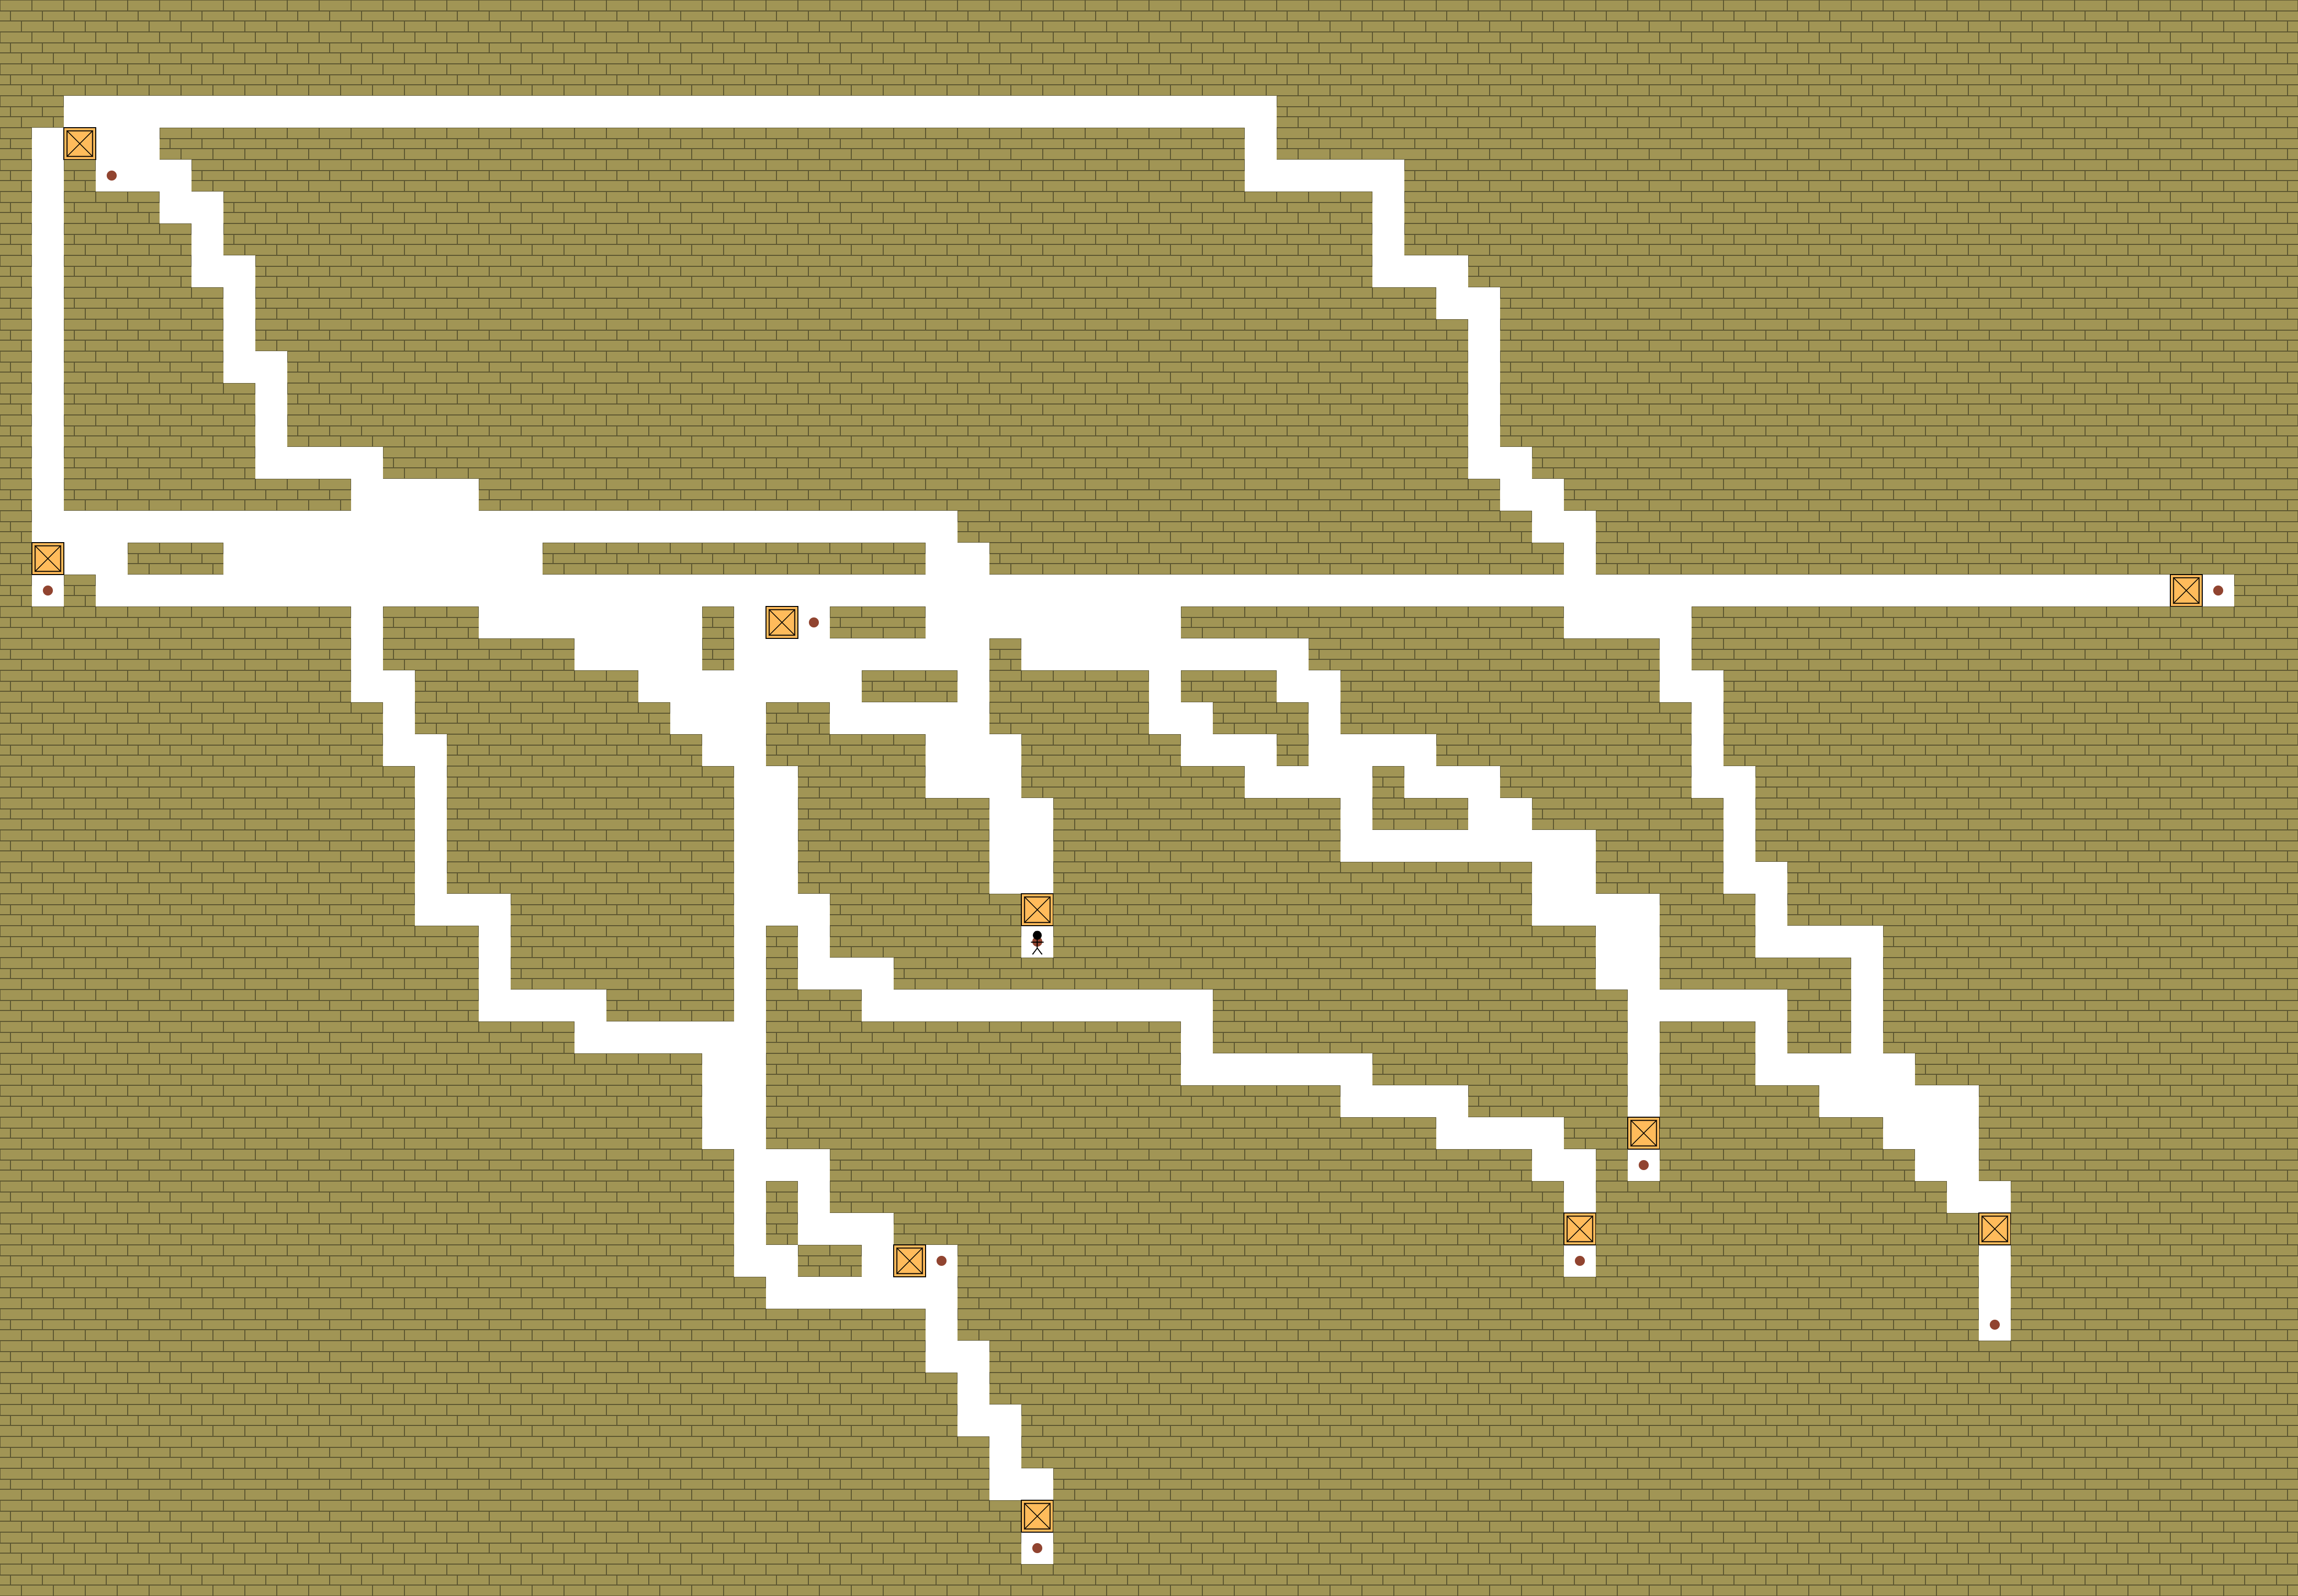
\includegraphics[width=\textwidth]{board_shape_full}
	\end{subfigure}
	\hspace{0.05\textwidth}
	\begin{subfigure}[b]{0.4\linewidth}
		\centering
		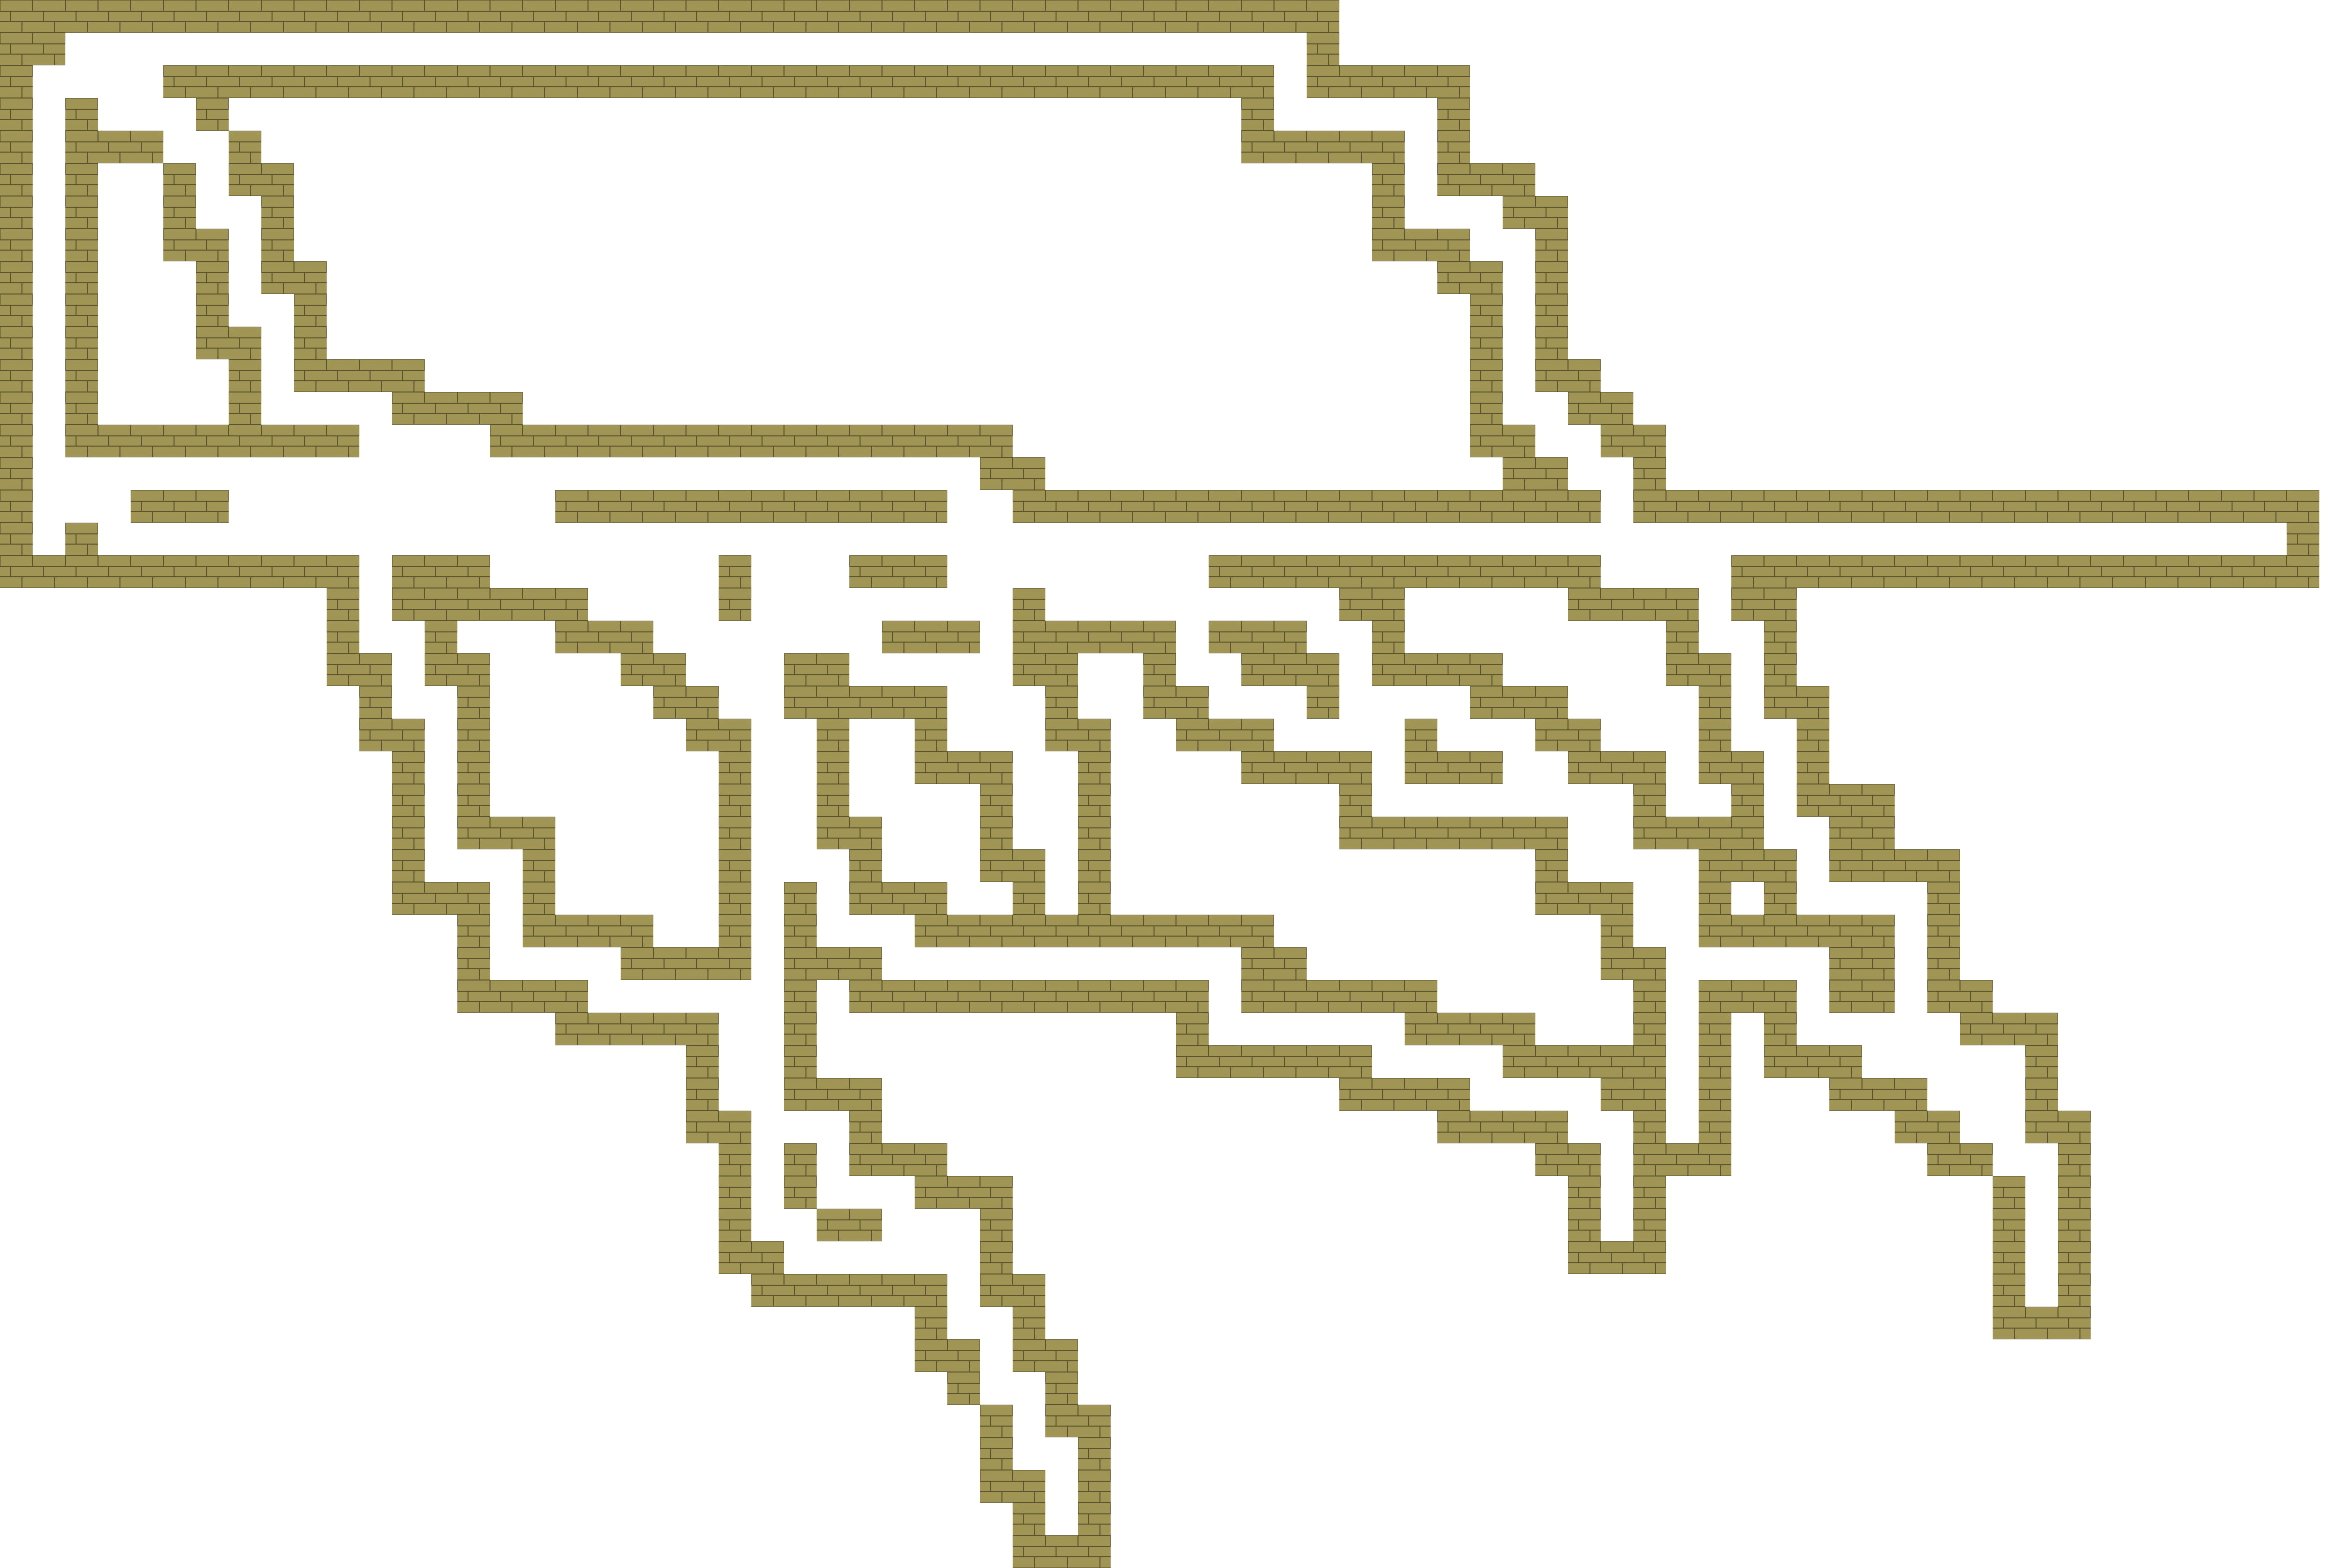
\includegraphics[width=\textwidth]{board_shape_only}
	\end{subfigure}
	\caption{Plansza i~odpowiadający jej kształt}
	\label{rys:ksztalt_planszy}
\end{figure}


W kontekście rozmiaru plansz, analizy prezentowane w~rozdz.~\ref{subs:exp_sym}--\ref{subs:exp_ppo} wykazały, że~metody heurystyczne są~w~stanie generować plansze o~dostatecznym skomplikowaniu większe niż $6x6$. Metody oparte na~uczeniu maszynowym wypadają w~tej materii istotnie gorzej.

